\section{Auswertung}
\label{sec:Auswertung}

%Siehe \autoref{fig:plot}!
\subsection{Verzögerungszeit}
\begin{table}
    \centering
    \caption{Die Anzahl detektierter Ereignisse in Abhängigkeit der eingestellten Verzögerungszeit $t$ der Verzögerungsleitungen.
    Eine Verzögerung auf der linken bzw. rechten Leitung entspricht negativen bzw. positiven Verzögerungszeiten.
    }
    \label{tab:verzoegerung}
    \begin{tabular}{cc|cc}
        \toprule
        $t \,/\, \unit{\nano\second}$ & Anzahl Impulse in $\qty{10}{\second}$ & $t \,/\, \unit{\nano\second}$ & Anzahl Impulse in $\qty{10}{\second}$ \\
        \midrule
        -28 & 0 & 1 & 215 \\
        -26 & 0 & 2 & 227 \\
        -24 & 0 & 3 & 237 \\
        -22 & 0 & 4 & 260 \\
        -20 & 1 & 6 & 281 \\
        -18 & 9 & 8 & 300 \\
        -16 & 10 & 10 & 255 \\
        -14 & 23 & 12 & 234 \\
        -12 & 35 & 14 & 162 \\
        -10 & 57 & 16 & 96 \\
        -8 & 99 & 18 & 75 \\
        -6 & 168 & 20 & 45 \\
        -4 & 183 & 22 & 25 \\
        -3 & 188 & 24 & 20 \\
        -2 & 205 & 26 & 10 \\
        -1 & 221 & 28 & 6 \\
        0 & 212 & & \\

        \bottomrule
    \end{tabular}
\end{table}

\begin{figure}
    \centering
    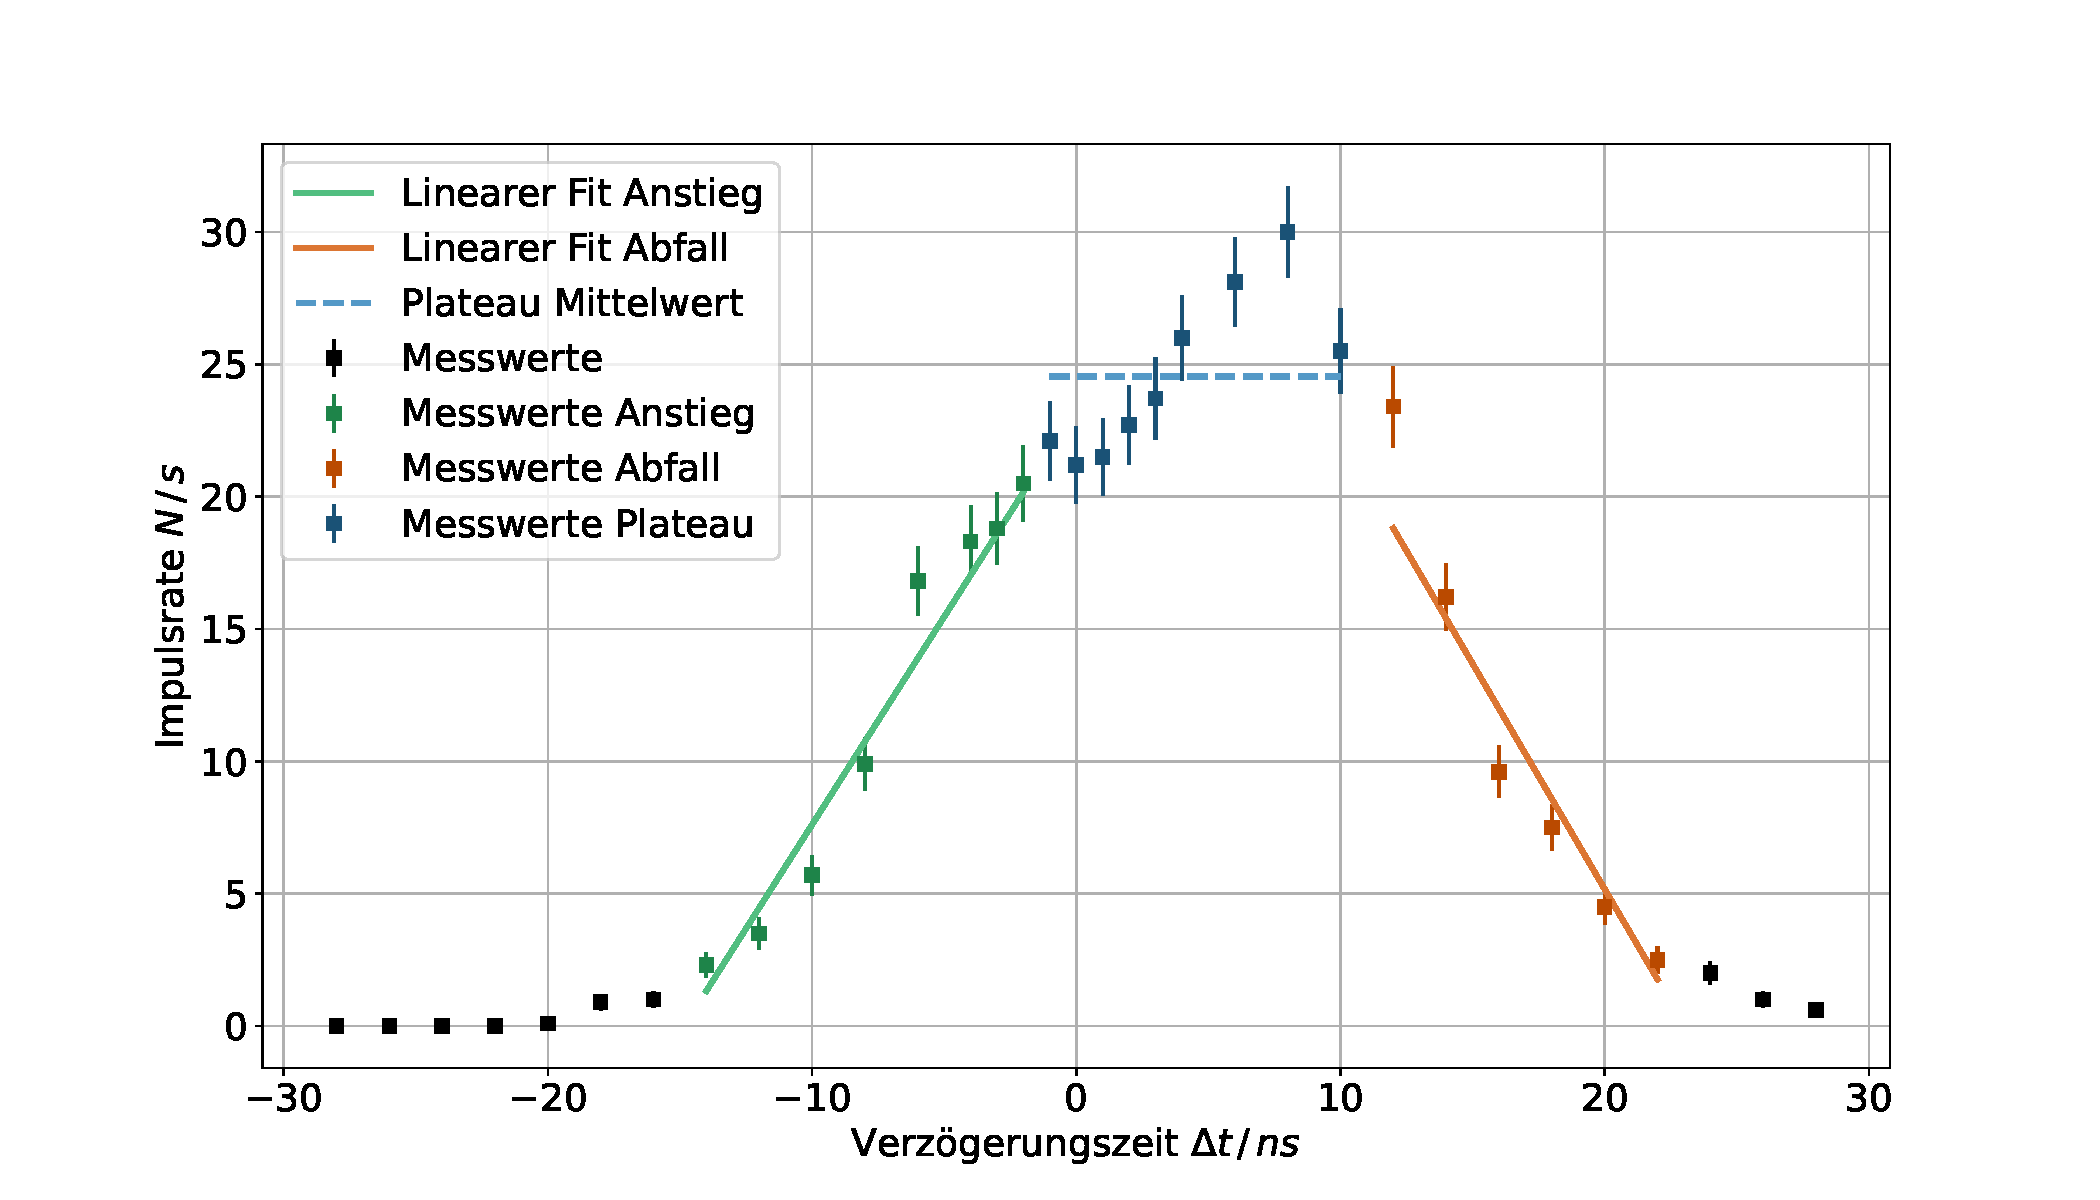
\includegraphics[width=0.8\textwidth]{content/plots/verzoegerungszeit.pdf}
    \caption{Die gemessene Ereignisrate $N$ in Abhängigkeit der Verzögerungszeit $\Delta t$.
    Die Messwerte werden in 3 Bereiche unterteilt, wobei die ersten und lette
    Der Anstieg und Abfall wird näherungsweise jeweils durch einen linearen Fit dargestellt.
    Das Mittel über die zum Plateau zugehörigen Messwerte definiert die Plateau-Höhe.}
    \label{fig:verzoegerung}
\end{figure}

\subsection{Kalibration}

\subsection{Statistische Abschätzung der Untergrundereignisse}

\subsection{Experimentell bestimmte Untergrundrate und Lebensdauer der Myonen}